\begin{frame}{}

  \vspace{1cm}
  \begin{figure}\centering
    \definecolor{c1}{rgb}{0 0.4470 0.7410}
\definecolor{c2}{rgb}{0.8500 0.3250 0.0980}
\definecolor{c3}{rgb}{0.9290 0.6940 0.1250}
\definecolor{c4}{rgb}{0.4940 0.1840 0.5560}
\definecolor{c5}{rgb}{0.4660 0.6740 0.1880}
\definecolor{c6}{rgb}{0.3010 0.7450 0.9330}
\definecolor{c7}{RGB}{251,180,185}
\definecolor{c8}{RGB}{247,104,161}
\definecolor{c9}{RGB}{255,0,255}

% GNUPLOT: LaTeX picture with Postscript
\begingroup
  \makeatletter
  \providecommand\color[2][]{%
    \GenericError{(gnuplot) \space\space\space\@spaces}{%
      Package color not loaded in conjunction with
      terminal option `colourtext'%
    }{See the gnuplot documentation for explanation.%
    }{Either use 'blacktext' in gnuplot or load the package
      color.sty in LaTeX.}%
    \renewcommand\color[2][]{}%
  }%
  \providecommand\includegraphics[2][]{%
    \GenericError{(gnuplot) \space\space\space\@spaces}{%
      Package graphicx or graphics not loaded%
    }{See the gnuplot documentation for explanation.%
    }{The gnuplot epslatex terminal needs graphicx.sty or graphics.sty.}%
    \renewcommand\includegraphics[2][]{}%
  }%
  \providecommand\rotatebox[2]{#2}%
  \@ifundefined{ifGPcolor}{%
    \newif\ifGPcolor
    \GPcolorfalse
  }{}%
  \@ifundefined{ifGPblacktext}{%
    \newif\ifGPblacktext
    \GPblacktexttrue
  }{}%
  % define a \g@addto@macro without @ in the name:
  \let\gplgaddtomacro\g@addto@macro
  % define empty templates for all commands taking text:
  \gdef\gplfronttext{}%
  \gdef\gplfronttext{}%
  \makeatother
  \ifGPblacktext
    % no textcolor at all
    \def\colorrgb#1{}%
    \def\colorgray#1{}%
  \else
    % gray or color?
    \ifGPcolor
      \def\colorrgb#1{\color[rgb]{#1}}%
      \def\colorgray#1{\color[gray]{#1}}%
      \expandafter\def\csname LTw\endcsname{\color{white}}%
      \expandafter\def\csname LTb\endcsname{\color{black}}%
      \expandafter\def\csname LTa\endcsname{\color{black}}%
      \expandafter\def\csname LT0\endcsname{\color[rgb]{1,0,0}}%
      \expandafter\def\csname LT1\endcsname{\color[rgb]{0,1,0}}%
      \expandafter\def\csname LT2\endcsname{\color[rgb]{0,0,1}}%
      \expandafter\def\csname LT3\endcsname{\color[rgb]{1,0,1}}%
      \expandafter\def\csname LT4\endcsname{\color[rgb]{0,1,1}}%
      \expandafter\def\csname LT5\endcsname{\color[rgb]{1,1,0}}%
      \expandafter\def\csname LT6\endcsname{\color[rgb]{0,0,0}}%
      \expandafter\def\csname LT7\endcsname{\color[rgb]{1,0.3,0}}%
      \expandafter\def\csname LT8\endcsname{\color[rgb]{0.5,0.5,0.5}}%
    \else
      % gray
      \def\colorrgb#1{\color{black}}%
      \def\colorgray#1{\color[gray]{#1}}%
      \expandafter\def\csname LTw\endcsname{\color{white}}%
      \expandafter\def\csname LTb\endcsname{\color{black}}%
      \expandafter\def\csname LTa\endcsname{\color{black}}%
      \expandafter\def\csname LT0\endcsname{\color{black}}%
      \expandafter\def\csname LT1\endcsname{\color{black}}%
      \expandafter\def\csname LT2\endcsname{\color{black}}%
      \expandafter\def\csname LT3\endcsname{\color{black}}%
      \expandafter\def\csname LT4\endcsname{\color{black}}%
      \expandafter\def\csname LT5\endcsname{\color{black}}%
      \expandafter\def\csname LT6\endcsname{\color{black}}%
      \expandafter\def\csname LT7\endcsname{\color{black}}%
      \expandafter\def\csname LT8\endcsname{\color{black}}%
    \fi
  \fi
    \setlength{\unitlength}{0.0500bp}%
    \ifx\gptboxheight\undefined%
      \newlength{\gptboxheight}%
      \newlength{\gptboxwidth}%
      \newsavebox{\gptboxtext}%
    \fi%
    \setlength{\fboxrule}{0.5pt}%
    \setlength{\fboxsep}{1pt}%
\begin{picture}(8000.00,4800.00)%
    \gplgaddtomacro\gplfronttext{%
      \colorrgb{0.15,0.15,0.15}%
      %\put(-52,2448){\makebox(0,0)[r]{\strut{}$40\%$}}%
      \colorrgb{0.15,0.15,0.15}%
      \put(-52,3216){\makebox(0,0)[r]{\strut{}$60\%$}}%
      \colorrgb{0.15,0.15,0.15}%
      \put(-52,3983){\makebox(0,0)[r]{\strut{}$80\%$}}%
      \colorrgb{0.15,0.15,0.15}%
      \put(-52,4751){\makebox(0,0)[r]{\strut{}$100\%$}}%
      \colorrgb{0.15,0.15,0.15}%
      \put(80,2228){\makebox(0,0){\strut{}}}%
      \colorrgb{0.15,0.15,0.15}%
      \put(439,2228){\makebox(0,0){\strut{}}}%
      \colorrgb{0.15,0.15,0.15}%
      \put(817,2228){\makebox(0,0){\strut{}}}%
      \colorrgb{0.15,0.15,0.15}%
      \put(1574,2228){\makebox(0,0){\strut{}}}%
    }%
    \gplgaddtomacro\gplfronttext{%
      \colorrgb{0.15,0.15,0.15}%
      \put(-718,3599){\rotatebox{90}{\makebox(0,0){\strut{}$\sigma_{\bm{M}} = 0.0$ m}}}%
      \colorrgb{0.00,0.00,0.00}%
      \put(831,4971){\makebox(0,0){\strut{}$\sigma_R = 0.01$ m}}%
      \put(3999,6200){\makebox(0,0){\strut{}Ποσοστό επιτυχίας στόχου (\ref{objective:02_04})}}%
      \put(3999,5900){\makebox(0,0){\strut{}ως προς θέση ανά μονάδα αρχικού σφάλματος εκτίμησης προσανατολισμού $\Delta\hat{\theta}$}}%
      \put(0,5400){\makebox(0,0){\strut{}{\color{c1}{\rule[0.6mm]{0.5cm}{0.5mm}}}PLICP}}
      \put(1000,5400){\makebox(0,0){\strut{}{\color{c2}{\rule[0.6mm]{0.5cm}{0.5mm}}}NDT}}
      \put(2000,5400){\makebox(0,0){\strut{}{\color{c3}{\rule[0.6mm]{0.5cm}{0.5mm}}}FastGICP}}
      \put(3400,5400){\makebox(0,0){\strut{}{\color{c4}{\rule[0.6mm]{0.5cm}{0.5mm}}}FastVGICP}}
      \put(4800,5400){\makebox(0,0){\strut{}{\color{c5}{\rule[0.6mm]{0.5cm}{0.5mm}}}NDT-PSO}}
      \put(6100,5400){\makebox(0,0){\strut{}{\color{c6}{\rule[0.6mm]{0.5cm}{0.5mm}}}TEASER}}
      \put(7000,5400){\makebox(0,0){\strut{}{\color{c7}{\rule[0.6mm]{0.5cm}{0.5mm}}}\texttt{x1}}}
      \put(7600,5400){\makebox(0,0){\strut{}{\color{c8}{\rule[0.6mm]{0.5cm}{0.5mm}}}\texttt{uf}}}
      \put(8200,5400){\makebox(0,0){\strut{}{\color{c9}{\rule[0.6mm]{0.5cm}{0.5mm}}}\texttt{fm}}}
      \put(3999,-550){\makebox(0,0){\strut{}Αρχικό σφάλμα εκτίμησης προσανατολισμού $|\Delta\hat{\theta}|$ [rad]}}%
    }%
    \gplgaddtomacro\gplfronttext{%
      \colorrgb{0.15,0.15,0.15}%
      \put(1532,2448){\makebox(0,0)[r]{\strut{}}}%
      \colorrgb{0.15,0.15,0.15}%
      \put(1532,3216){\makebox(0,0)[r]{\strut{}}}%
      \colorrgb{0.15,0.15,0.15}%
      \put(1532,3983){\makebox(0,0)[r]{\strut{}}}%
      \colorrgb{0.15,0.15,0.15}%
      \put(1532,4751){\makebox(0,0)[r]{\strut{}}}%
      \colorrgb{0.15,0.15,0.15}%
      \put(1664,2228){\makebox(0,0){\strut{}}}%
      \colorrgb{0.15,0.15,0.15}%
      \put(2023,2228){\makebox(0,0){\strut{}}}%
      \colorrgb{0.15,0.15,0.15}%
      \put(2401,2228){\makebox(0,0){\strut{}}}%
      \colorrgb{0.15,0.15,0.15}%
      \put(3158,2228){\makebox(0,0){\strut{}}}%
    }%
    \gplgaddtomacro\gplfronttext{%
      \colorrgb{0.00,0.00,0.00}%
      \put(2415,4971){\makebox(0,0){\strut{}$\sigma_R = 0.03$ m}}%
    }%
    \gplgaddtomacro\gplfronttext{%
      \colorrgb{0.15,0.15,0.15}%
      \put(3116,2448){\makebox(0,0)[r]{\strut{}}}%
      \colorrgb{0.15,0.15,0.15}%
      \put(3116,3216){\makebox(0,0)[r]{\strut{}}}%
      \colorrgb{0.15,0.15,0.15}%
      \put(3116,3983){\makebox(0,0)[r]{\strut{}}}%
      \colorrgb{0.15,0.15,0.15}%
      \put(3116,4751){\makebox(0,0)[r]{\strut{}}}%
      \colorrgb{0.15,0.15,0.15}%
      \put(3248,2228){\makebox(0,0){\strut{}}}%
      \colorrgb{0.15,0.15,0.15}%
      \put(3607,2228){\makebox(0,0){\strut{}}}%
      \colorrgb{0.15,0.15,0.15}%
      \put(3985,2228){\makebox(0,0){\strut{}}}%
      \colorrgb{0.15,0.15,0.15}%
      \put(4742,2228){\makebox(0,0){\strut{}}}%
    }%
    \gplgaddtomacro\gplfronttext{%
      \colorrgb{0.00,0.00,0.00}%
      \put(3999,4971){\makebox(0,0){\strut{}$\sigma_R = 0.05$ m}}%
    }%
    \gplgaddtomacro\gplfronttext{%
      \colorrgb{0.15,0.15,0.15}%
      \put(4700,2448){\makebox(0,0)[r]{\strut{}}}%
      \colorrgb{0.15,0.15,0.15}%
      \put(4700,3216){\makebox(0,0)[r]{\strut{}}}%
      \colorrgb{0.15,0.15,0.15}%
      \put(4700,3983){\makebox(0,0)[r]{\strut{}}}%
      \colorrgb{0.15,0.15,0.15}%
      \put(4700,4751){\makebox(0,0)[r]{\strut{}}}%
      \colorrgb{0.15,0.15,0.15}%
      \put(4832,2228){\makebox(0,0){\strut{}}}%
      \colorrgb{0.15,0.15,0.15}%
      \put(5191,2228){\makebox(0,0){\strut{}}}%
      \colorrgb{0.15,0.15,0.15}%
      \put(5569,2228){\makebox(0,0){\strut{}}}%
      \colorrgb{0.15,0.15,0.15}%
      \put(6326,2228){\makebox(0,0){\strut{}}}%
    }%
    \gplgaddtomacro\gplfronttext{%
      \colorrgb{0.00,0.00,0.00}%
      \put(5583,4971){\makebox(0,0){\strut{}$\sigma_R = 0.10$ m}}%
    }%
    \gplgaddtomacro\gplfronttext{%
      \colorrgb{0.15,0.15,0.15}%
      \put(6284,2448){\makebox(0,0)[r]{\strut{}}}%
      \colorrgb{0.15,0.15,0.15}%
      \put(6284,3216){\makebox(0,0)[r]{\strut{}}}%
      \colorrgb{0.15,0.15,0.15}%
      \put(6284,3983){\makebox(0,0)[r]{\strut{}}}%
      \colorrgb{0.15,0.15,0.15}%
      \put(6284,4751){\makebox(0,0)[r]{\strut{}}}%
      \colorrgb{0.15,0.15,0.15}%
      \put(6416,2228){\makebox(0,0){\strut{}}}%
      \colorrgb{0.15,0.15,0.15}%
      \put(6775,2228){\makebox(0,0){\strut{}}}%
      \colorrgb{0.15,0.15,0.15}%
      \put(7153,2228){\makebox(0,0){\strut{}}}%
      \colorrgb{0.15,0.15,0.15}%
      \put(7910,2228){\makebox(0,0){\strut{}}}%
    }%
    \gplgaddtomacro\gplfronttext{%
      \colorrgb{0.00,0.00,0.00}%
      \put(7167,4971){\makebox(0,0){\strut{}$\sigma_R = 0.20$ m}}%
    }%
    \gplgaddtomacro\gplfronttext{%
      \colorrgb{0.15,0.15,0.15}%
      \put(-52,48){\makebox(0,0)[r]{\strut{}$40\%$}}%
      \colorrgb{0.15,0.15,0.15}%
      \put(-52,816){\makebox(0,0)[r]{\strut{}$60\%$}}%
      \colorrgb{0.15,0.15,0.15}%
      \put(-52,1583){\makebox(0,0)[r]{\strut{}$80\%$}}%
      \colorrgb{0.15,0.15,0.15}%
      \put(-52,2351){\makebox(0,0)[r]{\strut{}$100\%$}}%
      \colorrgb{0.15,0.15,0.15}%
      \put(80,-172){\makebox(0,0){\strut{}$0.0$}}%
      \colorrgb{0.15,0.15,0.15}%
      \put(439,-172){\makebox(0,0){\strut{}$\frac{\pi}{16}$}}%
      \colorrgb{0.15,0.15,0.15}%
      \put(817,-172){\makebox(0,0){\strut{}$\frac{\pi}{8}$}}%
      \colorrgb{0.15,0.15,0.15}%
      \put(1574,-172){\makebox(0,0){\strut{}$\frac{\pi}{4}$}}%
    }%
    \gplgaddtomacro\gplfronttext{%
      \colorrgb{0.15,0.15,0.15}%
      \put(-718,1199){\rotatebox{90}{\makebox(0,0){\strut{}$\sigma_{\bm{M}} = 0.05$ m}}}%
    }%
    \gplgaddtomacro\gplfronttext{%
      \colorrgb{0.15,0.15,0.15}%
      \put(1532,48){\makebox(0,0)[r]{\strut{}}}%
      \colorrgb{0.15,0.15,0.15}%
      \put(1532,816){\makebox(0,0)[r]{\strut{}}}%
      \colorrgb{0.15,0.15,0.15}%
      \put(1532,1583){\makebox(0,0)[r]{\strut{}}}%
      \colorrgb{0.15,0.15,0.15}%
      \put(1532,2351){\makebox(0,0)[r]{\strut{}}}%
      \colorrgb{0.15,0.15,0.15}%
      %\put(1664,-172){\makebox(0,0){\strut{}$0.0$}}%
      \colorrgb{0.15,0.15,0.15}%
      \put(2023,-172){\makebox(0,0){\strut{}$\frac{\pi}{16}$}}%
      \colorrgb{0.15,0.15,0.15}%
      \put(2401,-172){\makebox(0,0){\strut{}$\frac{\pi}{8}$}}%
      \colorrgb{0.15,0.15,0.15}%
      \put(3158,-172){\makebox(0,0){\strut{}$\frac{\pi}{4}$}}%
    }%
    \gplgaddtomacro\gplfronttext{%
    }%
    \gplgaddtomacro\gplfronttext{%
      \colorrgb{0.15,0.15,0.15}%
      \put(3116,48){\makebox(0,0)[r]{\strut{}}}%
      \colorrgb{0.15,0.15,0.15}%
      \put(3116,816){\makebox(0,0)[r]{\strut{}}}%
      \colorrgb{0.15,0.15,0.15}%
      \put(3116,1583){\makebox(0,0)[r]{\strut{}}}%
      \colorrgb{0.15,0.15,0.15}%
      \put(3116,2351){\makebox(0,0)[r]{\strut{}}}%
      \colorrgb{0.15,0.15,0.15}%
      %\put(3248,-172){\makebox(0,0){\strut{}$0.0$}}%
      \colorrgb{0.15,0.15,0.15}%
      \put(3607,-172){\makebox(0,0){\strut{}$\frac{\pi}{16}$}}%
      \colorrgb{0.15,0.15,0.15}%
      \put(3985,-172){\makebox(0,0){\strut{}$\frac{\pi}{8}$}}%
      \colorrgb{0.15,0.15,0.15}%
      \put(4742,-172){\makebox(0,0){\strut{}$\frac{\pi}{4}$}}%
    }%
    \gplgaddtomacro\gplfronttext{%
    }%
    \gplgaddtomacro\gplfronttext{%
      \colorrgb{0.15,0.15,0.15}%
      \put(4700,48){\makebox(0,0)[r]{\strut{}}}%
      \colorrgb{0.15,0.15,0.15}%
      \put(4700,816){\makebox(0,0)[r]{\strut{}}}%
      \colorrgb{0.15,0.15,0.15}%
      \put(4700,1583){\makebox(0,0)[r]{\strut{}}}%
      \colorrgb{0.15,0.15,0.15}%
      \put(4700,2351){\makebox(0,0)[r]{\strut{}}}%
      \colorrgb{0.15,0.15,0.15}%
      %\put(4832,-172){\makebox(0,0){\strut{}$0.0$}}%
      \colorrgb{0.15,0.15,0.15}%
      \put(5191,-172){\makebox(0,0){\strut{}$\frac{\pi}{16}$}}%
      \colorrgb{0.15,0.15,0.15}%
      \put(5569,-172){\makebox(0,0){\strut{}$\frac{\pi}{8}$}}%
      \colorrgb{0.15,0.15,0.15}%
      \put(6326,-172){\makebox(0,0){\strut{}$\frac{\pi}{4}$}}%
    }%
    \gplgaddtomacro\gplfronttext{%
    }%
    \gplgaddtomacro\gplfronttext{%
      \colorrgb{0.15,0.15,0.15}%
      \put(6284,48){\makebox(0,0)[r]{\strut{}}}%
      \colorrgb{0.15,0.15,0.15}%
      \put(6284,816){\makebox(0,0)[r]{\strut{}}}%
      \colorrgb{0.15,0.15,0.15}%
      \put(6284,1583){\makebox(0,0)[r]{\strut{}}}%
      \colorrgb{0.15,0.15,0.15}%
      \put(6284,2351){\makebox(0,0)[r]{\strut{}}}%
      \colorrgb{0.15,0.15,0.15}%
      %\put(6416,-172){\makebox(0,0){\strut{}$0.0$}}%
      \colorrgb{0.15,0.15,0.15}%
      \put(6775,-172){\makebox(0,0){\strut{}$\frac{\pi}{16}$}}%
      \colorrgb{0.15,0.15,0.15}%
      \put(7153,-172){\makebox(0,0){\strut{}$\frac{\pi}{8}$}}%
      \colorrgb{0.15,0.15,0.15}%
      \put(7910,-172){\makebox(0,0){\strut{}$\frac{\pi}{4}$}}%
    }%
    \gplgaddtomacro\gplfronttext{%
    }%
    \put(0,0){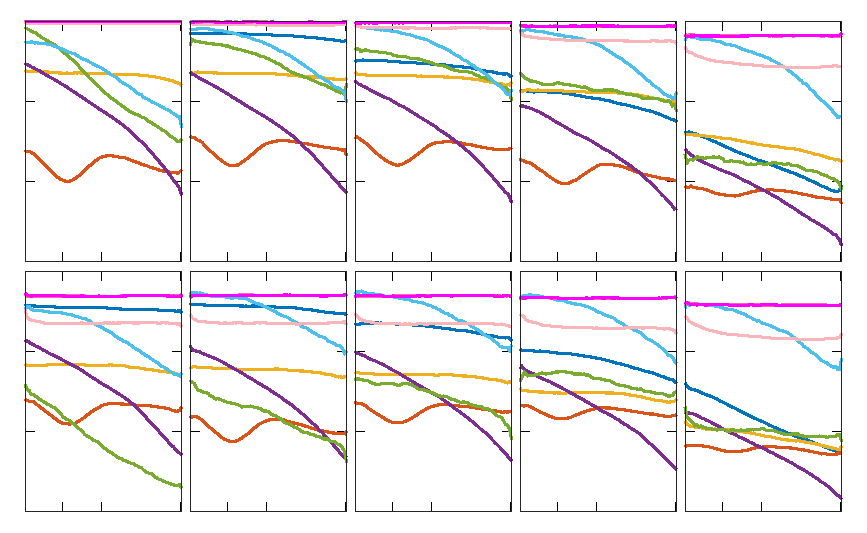
\includegraphics{./figures/parts/02/chapters/04/sections/05/cross_position_improvement_percent_orientation_binned_curves}}%
    \gplfronttext
  \end{picture}%
\endgroup

  \end{figure}


\note{\footnotesize
Κάπου εδώ θα τελείωνε η έρευνά μου, αλλά στο τέλος της έρευνάς μου είχα τη
διαίσθηση πως το γενικότερο πρόβλημα της ευθυγράμμισης πραγματικών σαρώσεων θα
μπορούσε να λυθεί μέσω της λύσης του προβλήματος της ευθυγράμμισης πραγματικών
με εικονικές σαρώσει}

\end{frame}
